%%%%%%%%%%%%%%%%%%%%%%%%%%%%%%%%%%%%%%%%%%%%%%%%%%%%%%%%%%%%%%%%%%%%%%%%
%                                                                      %
%     File: Thesis_Conclusion.tex                                    %
%     Tex Master: Thesis.tex                                           %
%                                                                      %
%     Author: Francisco Mendes                                           %
%     Last modified :  29 Dec 2019                                      %
%                                                                      %
%%%%%%%%%%%%%%%%%%%%%%%%%%%%%%%%%%%%%%%%%%%%%%%%%%%%%%%%%%%%%%%%%%%%%%%%

\chapter{Conclusion}
\label{chapter:conclusion}

The aim of this dissertation is to design a GPU DVFS aware mechanism, particularly tunned to the specificities of deep learning applications. Traditional GPU DVFS mechanisms are still considering the GPU as a black box, with little to no consideration about the executed workload.
The recent development of the ROC software stack, with software tools for independent voltage control, opens the possibility to explore the impacts of non-conventional DVFS parameters on GPGPU applications. However, these non conventional operating points can introduce faults on the system operation, mainly due to critical paths not being fulfilled or not sufficiently large voltage margin to accommodate the voltage noise. As a consequence, these faults can introduce small computation errors. However, there are applications that are highly tolerant to imprecision and as such, they can still operate correctly under these circumstances. One example of these applications is deep learning.

Under the described premise, this report has the objective of collecting the most relevant literature about GPU DVFS, power and performance modeling, as well as about deep learning applications. In Chapter 2, it is possible to get acquainted with the GPU architecture, and on how different types of applications respond to changes in the DVFS parameters. In Chapter 3, a description of the types of benchmarks that are going to be used is provided. They range from simple kernels that isolate the different GPU architectural components to fully-fledge, state-of-the-art, deep neural networks applications.  This description is followed by the feasibility assessments that were performed by running a CNN in severe undervoltage and maximum overclock scenarios. The preliminary results that were already obtained show that, mainly in the undervoltage scenario, it is possible to find more energy-efficient DVFS parameters if a correct tunning is applied during the DNN execution. One crucial detail is the confirmation that the set of network's weights, found in an overclock and undervoltage training scenario, are still valid for inference under conventional DVFS. Chapter 4, introduces the envisaged research that is going to be conducted during the dissertation. The set of identified tasks are represented in the Gantt chart of Figure \ref{fig:gantt}, that underlines the temporal relation between the objectives to be performed during this dissertation.

Overall, the literature review indicates that a DVFS exploration outside of the conventional operating points, focusing on the voltage space exploration, can lead to exciting results. In this way, the characterization, power and performance modeling and the creation of the DVFS aware mechanism that is proposed in this research plan is regarded as a highly attractive scientific path to be explored.

\begin{figure}[t!]
  \centering
  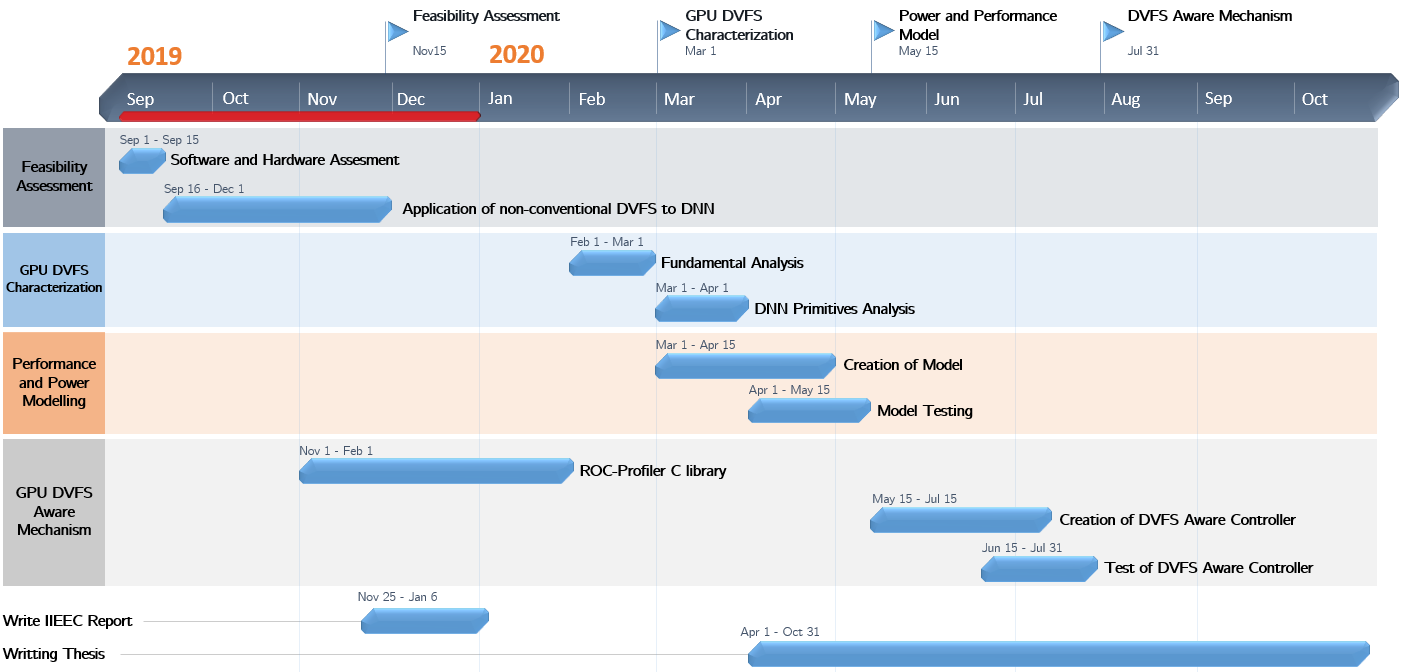
\includegraphics[width=1\textwidth]{Figures/Conclusion/Gantt.png}
  \caption[Conclusion]{Dissertation Gantt Chart.}
  \label{fig:gantt}
\end{figure}

